Last lecture we've looked at simple linear regression ($Y_i=\beta_0 + \beta_1x_i + \epsilon_i$)
\begin{center}
	\begin{tikzpicture}
	\begin{axis}[
	xmin=50, xmax=100, xlabel=temperature,
	ymin=100, ymax=250, ylabel=yiels,
	samples=400,
	axis x line=bottom,
	axis y line=left,
	domain=50:100,
	]
	\addplot[mark=x,only marks, blue] coordinates {
		(50,120)
		(53,115)
		(54,125)
		(55,119)
		(56,120)
		(59,140)
		(62,145)
		(64,143)
		(67,147)
		(71,157)
		(72,160)
		(74,175)
		(75,159)
		(76,177)
		(79,180)
		(80,185)
		(82,182)
		(85,185)
		(87,188)
		(89,200)
		(93,195)
		(94,203)
		(95,204)
		(97,212)
	};
	\end{axis}
	\end{tikzpicture}
\end{center}

This lecture we'll look at multiple linear regression (more than one predictor)
\begin{center}
		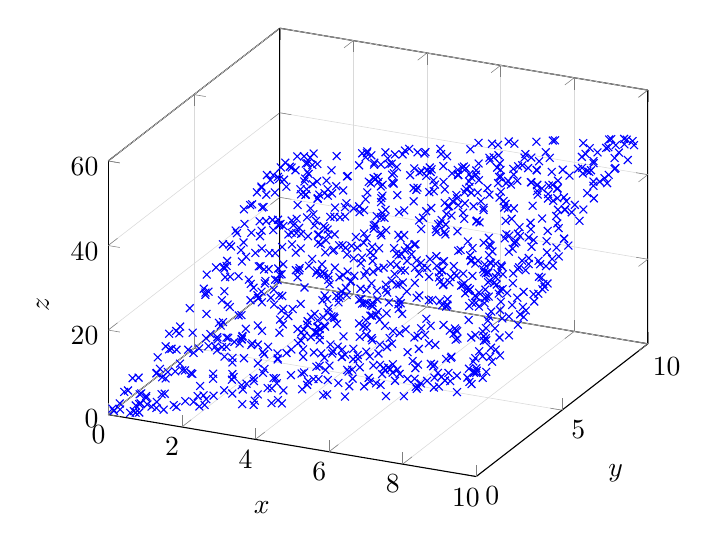
\begin{tikzpicture}
	\begin{axis}[
	xmin=0,xmax=10,xlabel=$x$,
	ymin=0,ymax=10,ylabel=$y$,
	zmin=0,zmax=60,zlabel=$z$,
	grid=both,
	grid style={line width=.2pt, draw=gray!30},
	%ytick={0,0.2,0.4,0.6,0.8,1},
	%ztick={0,0.2,0.4,0.6,0.8,1},
	]
	\addplot3[mark=x,only marks, blue] coordinates {
		(8.30,1.14,20.01)
		(8.49,7.96,40.87)
		(3.73,6.18,25.99)
		(5.93,0.70,13.97)
		(8.73,0.69,19.53)
		(9.34,1.36,22.75)
		(6.68,7.89,37.04)
		(2.07,0.92,6.91)
		(6.54,2.38,20.21)
		(0.72,2.44,8.75)
		(4.07,1.05,11.28)
		(6.67,8.58,39.09)
		(9.34,6.98,39.62)
		(8.11,7.34,38.23)
		(4.85,6.51,29.21)
		(7.57,5.16,30.62)
		(4.17,3.26,18.13)
		(9.72,6.62,39.29)
		(9.88,1.18,23.29)
		(8.64,1.48,21.72)
		(3.89,0.20,8.37)
		(4.55,9.64,38.02)
		(2.47,9.70,34.04)
		(7.84,1.24,19.40)
		(8.83,4.67,31.68)
		(9.14,6.57,37.98)
		(5.58,2.90,19.87)
		(5.99,7.55,34.61)
		(1.49,5.58,19.72)
		(9.00,4.28,30.83)
		(4.50,2.67,17.02)
		(2.06,7.54,26.73)
		(9.00,8.98,44.94)
		(7.63,7.28,37.11)
		(8.82,4.07,29.85)
		(2.85,9.38,33.85)
		(6.73,2.55,21.13)
		(6.64,5.33,29.28)
		(1.23,9.55,31.10)
		(4.07,2.68,16.18)
		(2.75,2.50,13.01)
		(7.17,9.28,42.16)
		(2.83,0.69,7.73)
		(8.96,2.99,26.91)
		(8.27,5.92,34.28)
		(3.90,2.03,13.90)
		(4.98,6.36,29.03)
		(6.95,7.98,37.85)
		(8.34,5.02,31.74)
		(6.10,6.51,31.72)
		(5.75,7.96,35.37)
		(3.26,2.33,13.52)
		(4.56,6.01,27.15)
		(7.14,1.12,17.65)
		(8.84,5.16,33.16)
		(7.21,8.38,39.55)
		(0.19,9.21,28.00)
		(6.75,4.98,28.44)
		(4.39,2.78,17.10)
		(4.38,6.53,28.33)
		(1.17,9.17,29.86)
		(8.15,5.10,31.59)
		(3.25,9.74,35.72)
		(2.46,1.97,10.84)
		(3.43,1.11,10.19)
		(3.76,2.97,16.43)
		(5.47,3.96,22.82)
		(5.62,4.21,23.86)
		(3.96,3.11,17.26)
		(3.98,6.94,28.78)
		(5.15,0.92,13.06)
		(6.58,4.02,25.21)
		(9.51,2.95,27.87)
		(7.22,3.06,23.64)
		(4.00,1.06,11.17)
		(8.32,5.94,34.45)
		(1.34,2.83,11.17)
		(0.60,1.55,5.87)
		(0.84,0.01,1.70)
		(1.64,2.84,11.79)
		(3.24,5.51,23.01)
		(3.02,8.71,32.16)
		(0.12,0.42,1.50)
		(5.40,9.05,37.94)
		(0.95,1.31,5.84)
		(1.47,8.34,27.94)
		(6.31,8.00,36.64)
		(8.59,9.18,44.72)
		(9.74,1.37,23.60)
		(5.71,5.05,26.56)
		(9.97,4.05,32.09)
		(5.54,1.74,16.28)
		(5.15,5.75,27.56)
		(3.31,6.06,24.80)
		(4.30,2.14,15.03)
		(4.92,5.20,25.43)
		(0.71,9.89,31.10)
		(8.88,4.90,32.45)
		(0.65,6.95,22.14)
		(4.36,4.11,21.07)
		(8.27,0.35,17.58)
		(3.95,2.93,16.68)
		(6.13,8.01,36.31)
		(8.19,3.47,26.77)
		(8.86,0.83,20.22)
		(9.31,5.11,33.96)
		(1.91,3.67,14.82)
		(2.59,7.39,27.36)
		(8.98,5.25,33.70)
		(5.93,8.05,36.00)
		(5.04,8.17,34.58)
		(6.13,1.89,17.94)
		(8.19,1.24,20.10)
		(5.32,8.21,35.27)
		(2.02,6.38,23.18)
		(4.54,0.16,9.56)
		(4.28,8.96,35.44)
		(9.66,5.15,34.78)
		(6.20,5.45,28.74)
		(6.95,6.06,32.10)
		(7.20,7.60,37.22)
		(3.47,8.55,32.60)
		(5.17,3.83,21.83)
		(5.57,0.85,13.67)
		(1.56,7.34,25.15)
		(5.62,3.32,21.20)
		(6.95,8.40,39.09)
		(4.26,3.72,19.68)
		(8.36,8.28,41.57)
		(7.31,1.77,19.92)
		(3.60,1.30,11.09)
		(4.54,8.80,35.48)
		(3.86,0.44,9.05)
		(7.76,6.87,36.11)
		(7.34,7.34,36.70)
		(4.30,4.37,21.72)
		(6.94,3.80,25.27)
		(9.45,9.80,48.29)
		(7.84,3.99,27.65)
		(7.06,4.40,27.32)
		(1.09,1.57,6.89)
		(3.90,3.26,17.58)
		(5.91,3.14,21.24)
		(4.59,8.95,36.02)
		(0.50,2.47,8.42)
		(2.29,3.11,13.89)
		(8.34,4.09,28.95)
		(0.16,7.08,21.55)
		(8.64,1.44,21.58)
		(0.78,8.71,27.70)
		(6.69,0.83,15.88)
		(5.00,4.62,23.86)
		(2.18,0.30,5.27)
		(5.72,7.53,34.03)
		(1.22,7.00,23.45)
		(6.71,2.15,19.86)
		(6.00,6.80,32.39)
		(0.56,5.57,17.84)
		(0.56,8.51,26.65)
		(1.53,5.59,19.81)
		(0.20,9.02,27.45)
		(4.35,4.20,21.29)
		(8.32,3.58,27.39)
		(6.17,4.89,27.02)
		(5.20,2.56,18.08)
		(8.64,9.29,45.15)
		(0.98,4.67,15.96)
		(9.08,2.54,25.78)
		(1.08,4.31,15.10)
		(5.17,7.03,31.42)
		(1.43,4.02,14.93)
		(5.59,1.82,16.64)
		(0.05,8.56,25.78)
		(7.67,5.84,32.86)
		(8.49,3.74,28.18)
		(9.17,2.22,24.99)
		(9.87,2.19,26.31)
		(5.05,5.22,25.77)
		(2.71,4.33,18.43)
		(1.01,7.41,24.25)
		(5.08,0.70,12.27)
		(5.86,8.47,37.13)
		(7.63,6.80,35.65)
		(0.83,1.37,5.76)
		(6.62,8.58,38.98)
		(5.17,2.00,16.33)
		(1.71,6.07,21.64)
		(9.39,5.43,35.06)
		(5.90,1.62,16.68)
		(4.41,0.06,8.98)
		(9.42,7.71,41.98)
		(6.56,7.65,36.06)
		(4.52,4.21,21.67)
		(8.40,0.57,18.50)
		(5.33,5.86,28.22)
		(5.54,1.74,16.30)
		(6.80,7.29,35.46)
		(3.67,5.34,23.37)
		(2.39,2.53,12.38)
		(5.79,9.17,39.09)
		(8.67,7.58,40.08)
		(4.07,8.87,34.75)
		(1.13,0.69,4.32)
		(4.44,1.84,14.38)
		(3.00,7.37,28.12)
		(4.01,6.97,28.93)
		(8.33,7.77,39.98)
		(4.04,5.02,23.13)
		(3.90,4.25,20.57)
		(3.60,6.11,25.55)
		(1.40,8.56,28.48)
		(2.60,6.71,25.33)
		(0.87,5.24,17.44)
		(4.29,2.99,17.55)
		(2.57,7.04,26.26)
		(2.98,3.82,17.40)
		(4.25,5.68,25.53)
		(1.19,8.88,29.02)
		(4.95,8.43,35.19)
		(7.06,8.99,41.09)
		(2.44,9.39,33.04)
		(7.85,8.15,40.16)
		(0.74,0.01,1.52)
		(3.94,0.03,7.97)
		(0.03,0.87,2.69)
		(2.21,2.61,12.24)
		(0.01,0.23,0.71)
		(1.89,4.24,16.51)
		(1.42,3.41,13.08)
		(2.68,5.41,21.60)
		(1.75,9.26,31.28)
		(1.39,2.98,11.73)
		(5.99,3.38,22.12)
		(9.01,8.59,43.81)
		(9.39,3.40,29.00)
		(2.21,1.38,8.57)
		(4.83,5.08,24.89)
		(3.76,8.57,33.22)
		(5.24,3.84,22.01)
		(2.65,6.96,26.17)
		(0.68,6.28,20.20)
		(4.36,4.50,22.24)
		(1.74,4.74,17.69)
		(0.26,9.50,29.01)
		(9.55,0.83,21.60)
		(4.31,2.80,17.01)
		(9.62,4.47,32.64)
		(7.62,5.88,32.88)
		(0.07,8.78,26.48)
		(6.80,4.69,27.67)
		(7.06,4.37,27.24)
		(6.45,7.46,35.29)
		(5.52,4.68,25.08)
		(2.18,8.61,30.19)
		(7.72,4.67,29.44)
		(2.28,4.98,19.50)
		(3.71,4.87,22.04)
		(8.91,2.29,24.70)
		(8.56,0.86,19.69)
		(4.02,0.67,10.07)
		(3.18,8.88,33.01)
		(6.09,2.33,19.17)
		(9.10,8.62,44.05)
		(9.09,7.12,39.53)
		(5.92,8.73,38.02)
		(3.33,9.38,34.79)
		(8.53,1.40,21.25)
		(4.42,3.94,20.66)
		(9.04,9.81,47.50)
		(0.33,6.45,20.01)
		(5.32,8.96,37.54)
		(7.16,4.82,28.80)
		(1.79,0.14,4.01)
		(3.37,6.23,25.42)
		(1.88,2.31,10.69)
		(3.22,5.27,22.26)
		(4.04,7.25,29.83)
		(5.49,6.07,29.19)
		(0.49,5.88,18.63)
		(5.53,4.33,24.06)
		(2.75,2.44,12.82)
		(2.42,4.29,17.70)
		(2.43,0.10,5.17)
		(1.54,6.09,21.35)
		(9.56,9.58,47.87)
		(9.36,0.95,21.58)
		(8.19,0.36,17.44)
		(7.28,8.86,41.15)
		(1.76,2.47,10.92)
		(3.60,0.09,7.47)
		(1.89,8.15,28.22)
		(0.01,1.40,4.24)
		(3.16,8.80,32.72)
		(7.00,0.95,16.85)
		(6.25,3.53,23.08)
		(5.43,5.93,28.66)
		(4.39,5.85,26.34)
		(2.87,6.68,25.78)
		(5.02,6.48,29.47)
		(7.62,4.33,28.23)
		(7.62,1.40,19.44)
		(5.76,7.52,34.08)
		(7.48,2.42,22.21)
		(6.46,6.50,32.42)
		(1.23,8.57,28.19)
		(5.04,0.84,12.62)
		(3.47,9.72,36.11)
		(0.92,0.31,2.79)
		(1.48,8.35,28.02)
		(1.98,8.36,29.03)
		(6.72,0.50,14.94)
		(4.32,5.46,25.01)
		(6.94,9.43,42.18)
		(2.57,3.21,14.78)
		(0.10,8.06,24.39)
		(5.32,6.01,28.69)
		(2.79,7.90,29.28)
		(9.46,7.99,42.90)
		(9.06,0.50,19.62)
		(3.93,2.83,16.35)
		(0.25,6.53,20.10)
		(6.71,4.90,28.12)
		(8.37,9.73,45.93)
		(9.71,7.48,41.88)
		(0.57,5.68,18.17)
		(4.50,2.99,17.98)
		(5.82,2.56,19.33)
		(6.87,8.87,40.33)
		(7.19,4.47,27.79)
		(6.50,8.16,37.48)
		(7.27,0.98,17.49)
		(3.74,8.60,33.26)
		(5.82,0.28,12.46)
		(1.16,8.99,29.30)
		(0.58,9.00,28.15)
		(9.80,5.24,35.32)
		(2.85,1.20,9.30)
		(5.95,1.78,17.23)
		(9.62,7.06,40.43)
		(1.86,8.31,28.66)
		(1.93,0.35,4.91)
		(3.42,7.58,29.57)
		(9.33,9.57,47.37)
		(3.91,3.43,18.10)
		(2.73,6.38,24.61)
		(1.52,3.43,13.33)
		(3.97,2.16,14.44)
		(3.75,7.86,31.08)
		(1.31,7.23,24.31)
		(4.35,2.79,17.07)
		(0.92,5.82,19.30)
		(6.15,4.21,24.92)
		(0.11,0.92,2.98)
		(5.73,0.24,12.19)
		(7.90,4.91,30.53)
		(2.35,2.78,13.06)
		(4.48,3.40,19.15)
		(5.69,2.87,20.01)
		(0.61,1.71,6.36)
		(4.96,3.99,21.90)
		(6.42,6.98,33.78)
		(2.21,2.04,10.54)
		(8.37,6.66,36.73)
		(9.71,4.43,32.71)
		(8.46,4.33,29.93)
		(5.06,1.75,15.38)
		(2.79,1.93,11.37)
		(7.47,6.16,33.42)
		(2.37,2.69,12.81)
		(9.57,5.60,35.94)
		(6.20,9.45,40.75)
		(6.00,7.14,33.44)
		(1.73,6.79,23.83)
		(0.90,9.59,30.59)
		(2.55,7.75,28.37)
		(8.59,6.08,35.40)
		(9.11,9.48,46.66)
		(7.00,0.60,15.78)
		(7.25,2.69,22.57)
		(2.30,9.87,34.20)
		(5.76,7.72,34.69)
		(8.11,4.75,30.47)
		(4.04,6.81,28.50)
		(9.88,4.17,32.28)
		(0.90,3.80,13.20)
		(3.21,2.13,12.82)
		(5.11,3.83,21.72)
		(0.61,0.30,2.10)
		(7.26,4.72,28.68)
		(5.57,3.33,21.13)
		(5.29,9.76,39.86)
		(8.30,5.55,33.26)
		(8.59,8.46,42.56)
		(7.89,4.08,28.02)
		(3.18,4.62,20.22)
		(4.52,8.26,33.83)
		(7.52,9.91,44.78)
		(1.10,5.24,17.92)
		(1.10,9.25,29.96)
		(2.70,7.39,27.57)
		(5.25,5.67,27.52)
		(9.73,9.69,48.52)
		(7.10,8.24,38.94)
		(3.12,9.60,35.03)
		(2.91,6.46,25.22)
		(8.50,3.80,28.39)
		(9.12,4.77,32.53)
		(6.39,9.12,40.14)
		(2.55,0.15,5.55)
		(0.89,1.57,6.47)
		(8.38,4.72,30.91)
		(5.85,5.43,27.98)
		(9.48,0.60,20.75)
		(0.61,6.58,20.96)
		(5.85,8.90,38.38)
		(2.85,1.10,8.99)
		(8.28,4.38,29.69)
		(1.91,2.80,12.23)
		(4.43,9.85,38.41)
		(3.93,6.09,26.13)
		(8.27,2.54,24.14)
		(6.77,1.33,17.52)
		(2.08,5.45,20.50)
		(3.18,8.28,31.20)
		(1.34,8.37,27.79)
		(6.71,8.33,38.43)
		(5.71,2.04,17.53)
		(1.70,5.44,19.73)
		(1.48,8.75,29.20)
		(4.76,1.21,13.15)
		(9.08,8.56,43.85)
		(5.52,9.00,38.04)
		(0.33,2.18,7.19)
		(0.54,0.77,3.39)
		(8.05,4.74,30.33)
		(4.51,8.35,34.08)
		(3.83,4.69,21.73)
		(7.90,4.14,28.21)
		(3.64,5.03,22.37)
		(5.32,1.25,14.41)
		(7.12,1.32,18.20)
		(8.71,8.70,43.54)
		(3.29,6.03,24.66)
		(6.50,2.65,20.96)
		(9.75,8.65,45.44)
		(0.76,0.58,3.26)
		(5.87,4.58,25.47)
		(4.14,7.22,29.94)
		(3.09,3.39,16.35)
		(2.64,4.01,17.31)
		(7.59,5.27,30.98)
		(9.95,8.94,46.73)
		(1.87,7.78,27.08)
		(7.81,0.69,17.70)
		(1.96,2.79,12.28)
		(9.92,3.79,31.23)
		(8.02,8.65,41.99)
		(4.24,4.20,21.08)
		(7.29,2.40,21.77)
		(4.98,5.98,27.90)
		(8.09,4.79,30.56)
		(3.57,8.99,34.09)
		(0.73,9.35,29.51)
		(5.91,8.18,36.36)
		(9.10,7.09,39.47)
		(1.94,7.43,26.17)
		(4.32,9.00,35.64)
		(7.49,0.65,16.94)
		(0.39,3.36,10.86)
		(9.46,0.04,19.06)
		(7.64,8.28,40.12)
		(5.59,5.07,26.40)
		(1.84,3.66,14.66)
		(4.98,2.27,16.76)
		(5.18,5.35,26.40)
		(9.94,2.89,28.57)
		(8.55,0.68,19.15)
		(9.62,0.85,21.80)
		(6.79,0.68,15.63)
		(4.04,4.10,20.36)
		(9.35,1.23,22.40)
		(4.79,4.43,22.88)
		(2.32,8.99,31.60)
		(3.96,3.54,18.53)
		(7.05,1.20,17.71)
		(5.59,5.69,28.24)
		(7.57,8.75,41.38)
		(9.95,3.49,30.37)
		(9.62,0.42,20.51)
		(5.35,1.42,14.97)
		(9.64,0.77,21.58)
		(1.16,7.41,24.53)
		(0.51,4.57,14.72)
		(3.04,6.68,26.13)
		(5.80,6.99,32.58)
		(5.31,5.71,27.76)
		(9.01,6.29,36.88)
		(5.41,8.78,37.14)
		(4.32,6.62,28.51)
		(5.43,8.75,37.12)
		(7.12,4.68,28.27)
		(0.17,1.41,4.57)
		(8.01,0.68,18.06)
		(1.43,7.14,24.28)
		(4.78,3.08,18.81)
		(2.57,6.71,25.27)
		(3.69,6.52,26.95)
		(6.62,5.31,29.17)
		(1.70,7.15,24.85)
		(2.79,5.05,20.72)
		(1.98,4.88,18.60)
		(1.95,4.98,18.84)
		(3.27,9.36,34.62)
		(8.80,3.89,29.29)
		(4.71,1.17,12.94)
		(4.04,2.40,15.29)
		(1.79,6.85,24.13)
		(9.69,8.39,44.56)
		(4.07,9.70,37.25)
		(8.44,2.15,23.34)
		(6.15,7.60,35.12)
		(3.77,5.84,25.06)
		(8.77,4.03,29.63)
		(7.85,5.10,31.00)
		(4.65,4.96,24.17)
		(8.14,6.51,35.82)
		(8.98,7.44,40.28)
		(4.29,3.02,17.64)
		(3.34,0.90,9.37)
		(5.97,8.26,36.71)
		(9.02,3.90,29.73)
		(7.02,7.75,37.30)
		(3.77,1.79,12.93)
		(7.35,1.09,17.98)
		(9.54,9.05,46.24)
		(5.43,8.76,37.15)
		(5.40,10.00,40.80)
		(3.11,8.64,32.15)
		(0.71,0.37,2.53)
		(1.82,5.45,19.98)
		(0.93,9.98,31.79)
		(4.63,5.11,24.60)
		(0.09,8.74,26.39)
		(9.15,0.70,20.41)
		(6.43,9.88,42.48)
		(0.01,9.23,27.71)
		(0.30,5.64,17.54)
		(2.08,4.31,17.11)
		(4.55,3.38,19.23)
		(1.27,7.21,24.17)
		(0.09,0.14,0.58)
		(7.27,3.74,25.76)
		(3.54,9.23,34.76)
		(7.80,5.46,32.00)
		(4.37,4.74,22.95)
		(4.37,4.97,23.63)
		(0.49,3.09,10.25)
		(0.50,9.51,29.52)
		(0.91,9.82,31.28)
		(5.94,5.14,27.29)
		(2.41,9.93,34.60)
		(8.41,4.56,30.50)
		(8.57,4.26,29.93)
		(9.64,2.13,25.67)
		(4.89,1.93,15.58)
		(2.20,8.33,29.39)
		(2.26,7.27,26.32)
		(5.37,5.30,26.63)
		(7.62,8.29,40.11)
		(3.48,5.12,22.31)
		(4.61,5.52,25.78)
		(6.39,2.13,19.19)
		(9.17,5.88,35.98)
		(1.62,1.43,7.51)
		(7.16,0.52,15.88)
		(5.78,6.83,32.05)
		(4.33,6.09,26.92)
		(8.84,2.20,24.27)
		(3.93,4.06,20.05)
		(1.79,6.30,22.48)
		(6.33,5.55,29.33)
		(6.24,1.28,16.31)
		(3.28,1.69,11.63)
		(8.03,0.01,16.09)
		(9.99,4.18,32.53)
		(9.81,4.88,34.27)
		(1.27,1.60,7.34)
		(2.32,6.67,24.65)
		(0.24,0.18,1.01)
		(6.07,1.20,15.74)
		(1.11,9.52,30.78)
		(4.07,9.76,37.42)
		(8.84,0.31,18.61)
		(5.48,4.94,25.78)
		(3.69,8.63,33.26)
		(2.08,2.43,11.45)
		(4.41,8.34,33.85)
		(9.56,8.14,43.53)
		(1.24,6.29,21.35)
		(4.71,0.02,9.48)
		(8.57,3.80,28.53)
		(0.43,9.04,28.00)
		(6.92,6.80,34.24)
		(9.79,3.79,30.94)
		(2.83,6.32,24.62)
		(1.34,2.43,9.97)
		(6.85,5.71,30.85)
		(9.09,9.82,47.64)
		(6.11,8.50,37.71)
		(9.00,2.83,26.50)
		(1.93,6.82,24.34)
		(7.54,3.58,25.83)
		(3.46,9.87,36.53)
		(4.19,0.84,10.89)
		(1.56,2.50,10.62)
		(8.19,8.11,40.72)
		(6.25,0.84,15.03)
		(7.39,5.31,30.71)
		(8.05,8.01,40.12)
		(0.67,7.39,23.51)
		(9.51,1.42,23.27)
		(4.98,4.38,23.09)
		(7.55,3.50,25.61)
		(7.42,4.78,29.20)
		(8.31,5.87,34.24)
		(1.57,1.46,7.50)
		(4.57,9.05,36.31)
		(6.18,6.40,31.57)
		(9.32,1.63,23.53)
		(8.35,5.66,33.68)
		(8.95,9.32,45.86)
		(5.83,7.83,35.14)
		(5.83,6.86,32.23)
		(8.55,4.66,31.09)
		(0.35,2.60,8.51)
		(8.85,5.69,34.79)
		(4.08,2.49,15.62)
		(0.36,3.19,10.31)
		(7.46,9.11,42.25)
		(1.55,8.85,29.65)
		(1.44,7.95,26.72)
		(6.06,9.26,39.89)
		(2.54,1.79,10.45)
		(3.24,5.18,22.01)
		(4.02,6.27,26.85)
		(4.06,9.13,35.52)
		(3.86,6.64,27.64)
		(6.10,3.89,23.87)
		(1.67,7.40,25.54)
		(1.88,8.18,28.29)
		(0.95,6.00,19.90)
		(3.23,0.85,9.01)
		(7.70,9.22,43.06)
		(2.34,0.54,6.29)
		(7.40,5.27,30.62)
		(6.93,1.19,17.42)
		(8.24,3.80,27.89)
		(8.28,8.13,40.94)
		(2.93,2.44,13.19)
		(3.09,8.84,32.72)
		(5.23,7.13,31.84)
		(3.25,3.78,17.85)
		(8.32,2.49,24.10)
		(8.10,2.53,23.79)
		(5.57,7.67,34.16)
		(2.63,0.50,6.76)
		(6.81,6.85,34.17)
		(2.34,6.20,23.28)
		(4.56,7.47,31.53)
		(3.85,9.77,37.01)
		(5.39,3.84,22.29)
		(9.92,2.60,27.64)
		(7.55,8.77,41.43)
		(9.80,8.06,43.79)
		(2.35,4.61,18.53)
		(5.29,0.91,13.30)
		(0.51,5.64,17.96)
		(7.57,1.87,20.76)
		(6.02,5.32,27.99)
		(8.57,3.55,27.79)
		(9.88,3.15,29.21)
		(9.29,7.27,40.39)
		(4.10,5.16,23.66)
		(0.00,7.91,23.73)
		(5.41,2.04,16.95)
		(2.08,6.78,24.50)
		(2.19,0.52,5.96)
		(3.26,8.01,30.55)
		(0.96,6.79,22.28)
		(7.48,9.46,43.33)
		(7.49,0.92,17.72)
		(5.43,9.08,38.12)
		(3.38,5.10,22.06)
		(8.32,6.15,35.09)
		(5.53,3.16,20.53)
		(9.58,0.77,21.48)
		(8.93,8.51,43.38)
		(3.57,1.45,11.47)
		(5.46,3.70,22.04)
		(3.47,6.22,25.61)
		(6.23,9.98,42.38)
		(7.97,5.17,31.45)
		(7.46,9.91,44.63)
		(1.26,2.27,9.31)
		(8.22,3.98,28.39)
		(0.25,6.97,21.40)
		(4.14,0.65,10.23)
		(7.31,7.48,37.06)
		(7.81,4.20,28.24)
		(3.67,8.11,31.69)
		(7.45,3.80,26.29)
		(8.92,3.19,27.42)
		(2.43,9.86,34.43)
		(1.30,7.18,24.14)
		(2.25,4.13,16.90)
		(3.50,0.99,9.96)
		(2.87,7.35,27.78)
		(9.27,6.37,37.67)
		(0.51,0.74,3.24)
		(5.93,1.21,15.47)
		(1.63,9.82,32.71)
		(8.38,4.97,31.67)
		(1.68,0.22,4.02)
		(5.02,0.54,11.66)
		(9.99,1.41,24.21)
		(3.55,8.93,33.91)
		(0.47,4.66,14.92)
		(2.14,5.61,21.10)
		(3.98,4.94,22.79)
		(3.34,0.68,8.71)
		(2.30,8.98,31.52)
		(9.36,2.89,27.38)
		(6.83,2.69,21.74)
		(9.62,5.94,37.07)
		(4.38,4.76,23.04)
		(9.40,3.68,29.86)
		(0.06,6.56,19.79)
		(6.10,9.38,40.35)
		(8.01,6.20,34.63)
		(2.33,2.83,13.14)
		(9.32,2.05,24.80)
		(7.63,4.39,28.44)
		(8.26,0.27,17.35)
		(5.73,8.76,37.75)
		(7.93,6.10,34.15)
		(3.29,2.04,12.69)
		(2.23,5.20,20.07)
		(3.12,0.54,7.86)
		(5.85,8.62,37.56)
		(8.30,4.43,29.89)
		(2.90,5.48,22.25)
		(4.03,5.67,25.06)
		(8.62,6.80,37.65)
		(6.15,3.71,23.44)
		(9.91,0.78,22.17)
		(2.04,4.56,17.76)
		(8.27,0.48,17.98)
		(6.76,7.38,35.66)
		(2.49,0.38,6.12)
		(4.76,9.54,38.14)
		(3.99,7.42,30.25)
		(5.99,9.37,40.11)
		(8.01,5.13,31.41)
		(1.05,2.41,9.33)
		(8.21,2.60,24.23)
		(8.41,7.59,39.59)
		(3.55,9.93,36.89)
		(4.30,3.57,19.30)
		(5.72,7.53,34.03)
		(7.01,1.10,17.32)
		(7.42,5.97,32.76)
		(7.58,4.31,28.08)
		(3.89,7.31,29.70)
		(4.29,2.61,16.42)
		(9.56,0.95,21.97)
		(5.73,4.51,24.99)
		(8.50,6.40,36.20)
		(2.76,1.32,9.49)
		(6.22,4.53,26.03)
		(5.88,6.52,31.33)
		(9.63,8.27,44.08)
		(0.86,3.08,10.96)
		(5.00,4.02,22.08)
		(5.22,8.84,36.96)
		(0.90,7.01,22.82)
		(9.05,2.42,25.35)
		(8.84,7.60,40.48)
		(4.39,2.91,17.51)
		(7.82,2.77,23.96)
		(1.48,0.06,3.15)
		(6.20,3.75,23.64)
		(2.61,4.37,18.32)
		(4.46,3.04,18.04)
		(8.44,2.91,25.61)
		(1.96,2.43,11.20)
		(3.04,9.37,34.18)
		(4.83,8.60,35.47)
		(3.38,3.97,18.67)
		(7.98,4.79,30.35)
		(9.87,5.65,36.70)
		(1.59,4.90,17.87)
		(2.37,2.70,12.83)
		(7.02,9.90,43.74)
		(3.75,1.84,13.02)
		(9.74,8.62,45.32)
		(9.72,0.33,20.43)
		(6.44,3.32,22.83)
		(8.60,7.49,39.66)
		(4.02,6.44,27.37)
		(6.32,1.69,17.72)
		(9.85,9.52,48.27)
		(5.59,5.43,27.49)
		(9.34,2.51,26.21)
		(7.20,5.79,31.76)
		(4.84,9.15,37.15)
		(6.39,8.96,39.65)
		(8.88,4.83,32.23)
		(1.99,4.43,17.26)
		(3.95,3.12,17.26)
		(9.92,0.55,21.50)
		(4.02,7.54,30.66)
		(6.59,1.32,17.14)
		(9.01,3.56,28.70)
		(9.95,3.96,31.78)
		(6.53,8.86,39.63)
		(1.08,0.21,2.81)
		(0.36,8.44,26.04)
		(6.18,2.88,21.00)
		(5.67,2.50,18.85)
		(9.62,4.88,33.89)
		(7.46,7.29,36.79)
		(6.63,2.03,19.33)
		(5.23,2.16,16.95)
		(2.60,9.76,34.49)
		(9.62,5.93,37.04)
		(5.40,3.04,19.94)
		(0.30,9.68,29.64)
		(6.96,8.96,40.81)
		(5.20,1.90,16.10)
		(0.59,0.02,1.23)
		(8.90,7.12,39.15)
		(3.30,8.68,32.64)
		(2.30,1.18,8.14)
		(1.14,0.39,3.45)
		(3.11,5.98,24.16)
		(2.28,6.04,22.70)
		(6.52,5.16,28.53)
		(0.66,0.08,1.55)
		(2.75,6.89,26.18)
		(2.82,9.46,34.02)
		(8.80,8.74,43.81)
		(4.44,1.13,12.28)
		(7.56,3.55,25.76)
		(6.03,2.42,19.32)
		(7.83,5.60,32.48)
		(1.14,6.13,20.66)
		(9.79,3.01,28.60)
		(8.49,7.98,40.92)
		(0.51,7.96,24.88)
		(4.66,7.81,32.76)
		(3.26,3.51,17.05)
		(6.30,0.54,14.23)
		(2.30,7.09,25.87)
		(5.80,9.93,41.39)
		(6.03,1.62,16.94)
		(6.00,1.14,15.40)
		(4.48,9.13,36.35)
		(0.35,4.82,15.16)
		(5.14,8.52,35.83)
		(4.08,8.10,32.45)
		(1.08,1.87,7.76)
		(4.60,2.47,16.61)
		(4.51,0.54,10.64)
		(5.51,6.09,29.29)
		(8.05,7.77,39.43)
		(7.01,5.11,29.35)
		(8.72,0.28,18.28)
		(0.52,9.90,30.76)
		(2.20,5.01,19.42)
		(4.60,3.32,19.15)
		(9.59,1.74,24.39)
		(7.90,6.26,34.57)
		(4.52,5.75,26.29)
		(3.33,7.51,29.20)
		(0.59,1.54,5.79)
		(7.41,3.57,25.52)
		(5.07,1.44,14.45)
		(2.00,8.51,29.52)
		(4.27,3.38,18.68)
		(1.69,2.75,11.63)
		(7.52,0.06,15.21)
		(3.68,8.02,31.42)
		(9.42,4.97,33.76)
		(0.17,5.38,16.48)
		(8.29,8.71,42.71)
		(6.27,7.23,34.22)
		(5.39,6.68,30.82)
		(6.51,1.79,18.37)
		(7.27,5.50,31.05)
		(0.94,9.60,30.69)
		(8.78,5.96,35.43)
		(0.14,8.09,24.54)
		(2.94,9.85,35.42)
		(1.80,8.86,30.18)
		(9.26,2.14,24.94)
		(0.68,0.35,2.40)
		(5.81,4.51,25.16)
		(6.37,0.14,13.16)
		(6.51,4.74,27.24)
		(8.65,9.51,45.83)
		(0.56,2.49,8.59)
		(8.17,3.86,27.93)
		(5.29,4.31,23.52)
		(6.94,8.31,38.81)
		(2.12,8.25,28.99)
		(5.43,4.53,24.46)
		(7.03,3.81,25.47)
		(9.56,9.26,46.90)
		(4.45,7.41,31.12)
		(0.85,7.38,23.84)
		(0.57,9.47,29.55)
		(6.29,5.10,27.89)
		(7.96,7.92,39.68)
		(6.91,4.52,27.39)
		(3.45,8.49,32.38)
		(9.47,3.90,30.65)
		(5.20,7.38,32.56)
		(9.54,9.76,48.37)
		(0.74,5.23,17.17)
		(2.07,4.30,17.04)
		(7.75,2.07,21.72)
		(9.14,3.23,27.99)
		(7.83,1.11,18.98)
		(2.96,3.75,17.17)
		(1.52,3.30,12.93)
		(8.48,3.42,27.22)
		(7.85,8.17,40.21)
		(2.71,5.32,21.37)
		(2.28,5.21,20.19)
		(3.21,7.74,29.65)
		(8.30,1.20,20.20)
		(8.22,6.25,35.21)
		(5.71,3.47,21.81)
		(5.72,3.35,21.48)
		(2.86,5.75,22.96)
		(6.99,8.64,39.90)
		(7.96,1.99,21.88)
		(4.42,6.72,29.01)
		(4.46,9.02,35.98)
		(4.66,1.99,15.29)
		(2.79,2.98,14.53)
		(6.75,4.97,28.40)
		(9.04,8.90,44.77)
		(9.09,5.01,33.21)
		(7.47,2.77,23.25)
		(2.61,5.34,21.23)
		(6.90,5.74,31.02)
		(1.32,4.13,15.02)
		(1.24,0.15,2.91)
		(1.91,7.03,24.90)
		(1.46,5.07,18.12)
		(5.85,3.81,23.14)
		(0.73,0.65,3.42)
		(8.22,3.59,27.20)
		(7.23,2.34,21.49)
		(9.26,2.04,24.62)
		(4.93,8.14,34.27)
		(6.55,3.93,24.90)
		(8.90,0.54,19.41)
		(5.39,3.75,22.02)
		(2.82,7.75,28.89)
		(9.76,1.65,24.48)
		(0.36,9.12,28.10)
		(3.26,3.19,16.10)
		(9.73,3.30,29.35)
		(3.65,2.04,13.43)
		(3.09,7.67,29.20)
		(1.21,0.70,4.52)
		(9.16,9.50,46.82)
		(1.35,1.58,7.46)
		(3.32,2.86,15.24)
		(8.97,6.87,38.56)
		(5.00,1.41,14.23)
		(6.15,5.12,27.67)
		(5.83,7.21,33.30)
		(6.98,9.29,41.83)
		(0.29,7.32,22.55)
		(5.28,7.50,33.05)
		(0.32,4.07,12.86)
		(8.27,2.39,23.73)
		(3.40,5.21,22.43)
		(8.47,2.19,23.51)
		(2.46,8.42,30.19)
		(5.81,6.63,31.52)
		(9.38,8.16,43.24)
		(0.48,7.94,24.77)
		(0.54,4.69,15.15)
		(0.21,3.10,9.70)
		(6.81,6.88,34.26)
		(5.99,9.87,41.58)
	};
	\end{axis}
	\end{tikzpicture}
\end{center}

\subsection{Structure of multiple linear regression models}

Good news: simple linear models are a special case of \begriff{multiple linear regression} and with minor extensions everything we've looked at so far still applies. For $p$ predictors and data tuples $\{(x_{1i},x_{2i},...,x_{pi},Y_i)\mid i=1,...,n\}$, we assume the relationship
\begin{align}
	Y_i = \beta_0 + \sum_{j=1}^{p} \beta_jx_{ji} + \epsilon_i\notag
\end{align}
As before, we assume $\epsilon_i\overset{i.i.d}{\sim}Normal(0,\sigma)$. 

The matrix notation, $Y=X\beta + \epsilon$, now becomes very convenient:
\begin{align}
	Y = \begin{pmatrix}
		Y_1 \\ \vdots \\ Y_n
	\end{pmatrix}\quad X = \begin{pmatrix}
		1 & x_{11} & \dots & x_{p1} \\ \vdots & \vdots & \vdots & \vdots \\ 1 & x_{1n} & \dots &  x_{pn}
	\end{pmatrix} \quad \beta = \begin{pmatrix}
		\beta_0 \\ \vdots \\ \beta_p
	\end{pmatrix}\quad \epsilon = \begin{pmatrix}
		\epsilon_1 \\ \vdots \\ \epsilon_n
	\end{pmatrix} \notag
\end{align}

As before, the random variable notation is
\begin{align}
	Y_i &\overset{i.i.d}{\sim} Normal\left(\beta_0 + \sum_{j=1}^{p} \beta_jx_{ji},\sigma\right) \notag \\
	Y &\sim Normal(X\beta,\mathbbm{1}\sigma) \notag
\end{align}

Model fitting using Maximum Likelihood Estimation (MLE) proceeds in the same way as for simple linear models seen before and is equivalent to Ordinary Least Squares (OLS) fitting. The likelihood function is given by
\begin{align}
	L(\beta\mid X) = \prod_{i=1}^n f_{Normal}\left(Y_i,\mu=\beta_0+\sum_{j=1}^{p} \beta_jx_{ji},\sigma\right)\notag
\end{align}
where $f_{Normal}$ is the PDF for the normal distribution evaluated at $Y_i$. The exact equations for parameter MLEs are
\begin{align}
	\label{MLR_parameter_estimates}
	\begin{split}
		\hat{\beta} &= (X^TX)^{-1}X^TY \\
		\hat{\sigma}^2 &= \frac{1}{n-(p+1)}(Y-X\hat{\beta})^T(Y-X\hat{\beta})
	\end{split}
\end{align}
Fitted values for the response are: $\hat{Y} = X\hat{\beta}$. Parameter estimates for one explanatory variable describe the relationship between this variable and the response variable when all other explanatory variables are held fixed.

\subsection{Assumptions of linear models}

The assumptions for multiple linear regression models are the same as for simple linear models:
\begin{itemize}
	\item \textbf{Linearity:} response variable is a linear combination of the explanatory variables
	\item \textbf{Normality:} errors follow a normal distribution
	\item \textbf{Homoscedasticity:} variance of the response variable (or errors) is constant.
	\item \textbf{Independence:} the errors are uncorrelated (ideally statistically independent).
	\item \textbf{Weak exogeneity:} the explanatory variables can be treated as fixed values, rather than random variables.
\end{itemize}
However, there is one important addition:
\begin{itemize}
	\item \textbf{Lack of perfect multicollinearity:} if two explanatory variables are perfectly correlated, we can not solve the equation for parameter estimates (\cref{MLR_parameter_estimates}). Some (but not perfect!) correlation between explanatory variables my be permissible.
\end{itemize}

\subsection{Hypothesis testing on linear model parameters}

Using a conceptionally similar approach as for simple linear models, we can test hypothesis about the $\beta$s and construct confidence intervals for them. Importantly, the test statistics depend on the entries of the matrix
\begin{align}
	(X^TX)^{-1} = \begin{pmatrix}
		c_{00} & c_{01} & \dots & c_{0p} \\ \vdots & \vdots & \vdots & \vdots \\ c_{p0} & c_{p1} & \dots & c_{pp}
	\end{pmatrix}\notag
\end{align}
as $\sigma_{\hat{\beta_j}}=\hat{\sigma}\cdot\sqrt{c_{jj}}$ ($j=1,...,p$). Off-diagonal entries determine the covariance of estimates and are important for the variance in prediction. Generally, $\sigma$ needs to be estimated, so in practise we use \person{Student}'s t-distribution and the test statistic
\begin{align}
	t = \frac{\hat{\beta_j}-\text{hypothesised value}}{\hat{\sigma}\sqrt{c_{jj}}} \notag
\end{align}
\textcolor{red}{Many details omitted - software does the work for us!}

\subsection{Model selection}

With the more general Linear Model formulation, we can create many different models. How to choose which model to use?

\begin{example}
	Consider the range of electric vehicles.
	\begin{center}
		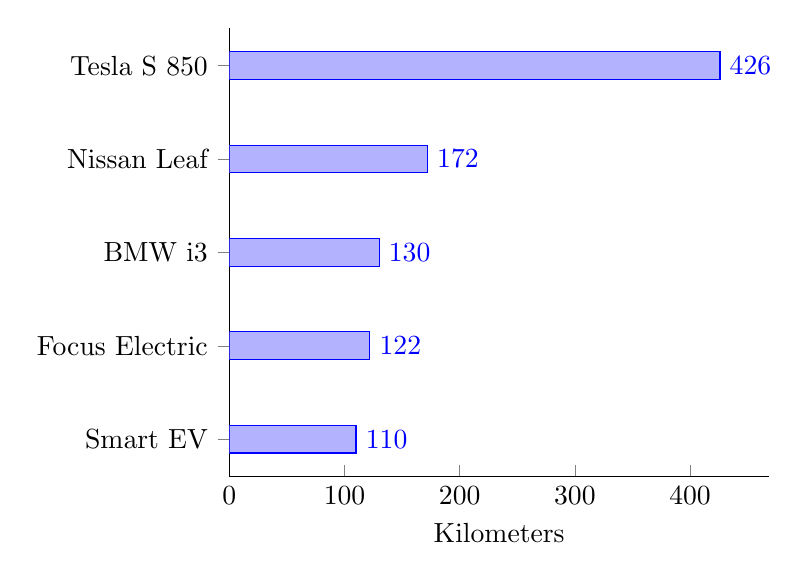
\begin{tikzpicture}
		\begin{axis}[ 
		xbar, xmin=0,
		xlabel={Kilometers},
		axis lines*=left,
		symbolic y coords={%
			{Smart EV},
			{Focus Electric},
			{BMW i3},
			{Nissan Leaf},
			{Tesla S 850}},
		ytick=data,
		nodes near coords, 
		nodes near coords align={horizontal},
		ytick=data,
		]
		\addplot coordinates {
			(110,{Smart EV}) 
			(122,{Focus Electric}) 
			(130,{BMW i3}) 
			(172,{Nissan Leaf})
			(426,{Tesla S 850})};
		\end{axis}
		\end{tikzpicture}
	\end{center}
	Depends on battery size, driving style or ambient temperature? Or all factors?
\end{example}

The right model depends on the purpose: Find all relevant factors? Prediction of range on a given day?

There is not one correct approach to model selection. What makes a good model depends on what it is designed for. Consequently, there are may different tools and techniques. Broadly, there are three types of model selection approaches:
\begin{itemize}
	\item Hypothesis tests on model parameters within models (include/exclude parameters).
	\item Measures that describe the quality or goodness of fit of models.
	\item Hypothesis tests comparing the fit of entire models (often related to measures from the previous point).
\end{itemize}
Fundamentally, model selection is at the heart of scientific inquiry. Statistical techniques offer one quantitative and rigorous approach. We'll go through a few of the most common statistical techniques.

\subsubsection{Hypothesis tests on model parameters}

We've encountered these already (test $H_0$: $\beta_j=0$). Could determine our model by fitting a full model that includes all conceivable explanatory variables first and than removing the explanatory variables for which we can't reject $H_0$.

\textbf{Problems:}
\begin{itemize}
	\item Multiple comparisons: conducting many hypothesis tests means that some may be rejected/accepted by chance (there are ways of dealing with this, e.g. \person{Bonferroni} correction).
	\item The model fit changes every time we remove an explanatory variable.
\end{itemize} 

While these tests are useful, we may want other approaches that allow us to test global hypotheses about models.

\subsubsection{$R^2$ and adjusted $R^2$}

\subsubsection{F-test on linear models}

\subsubsection{Quality measures based on the likelihood}

\subsubsection{Likelihood-ratio test for nested models}

\subsection{Automated or standardised model selection strategies}